\section{Page d'accueil des administrateurs}
\label{sec::home_admin}

\begin{figure}[H]
	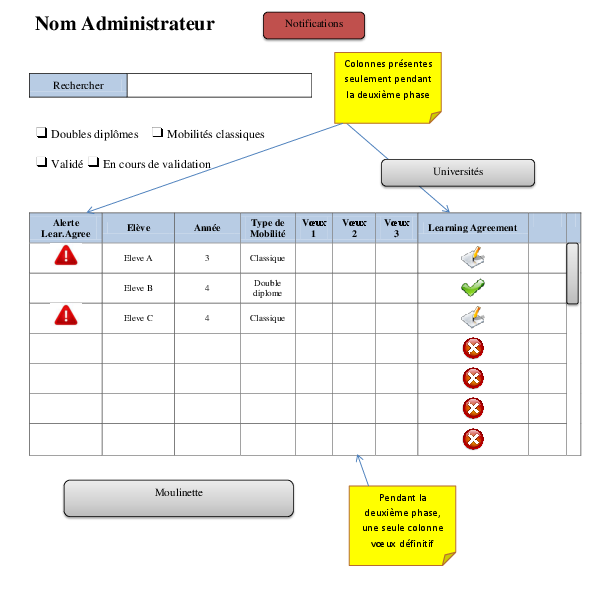
\includegraphics[scale=0.7]{Admin/HomeAd.png}
	\caption{Page d'accueil des administrateurs}
	\label{fig::hpa1}
\end{figure}

La figure \ref{fig::hpa1} représente la page sur laquelle un administrateur arrive après sa connexion au CAS. Cette page va servir à gérer les vœux des élèves lors de la première phase mais aussi les documents déposés par les élèves lors de la seconde.

Le principal élément de cette page est un tableau regroupant:
\begin{itemize}
 	\item le nom de l'élève ;
 	\item l'année de l'élève ;
 	\item si l'élève souhaite une mobilité classique ou double diplôme ;
 	\item une case précisant si les vœux de l'élève sont définitifs ou non (en phase 1) ;
 	\item une case précisant l'état de l'élève (Learning Agreement en attente, en cours de validation, validé) (en phase 2) ;
 	\item la liste des \voe de l'élève (en phase 1) ;
 	\item le \voe de l'élève (en phase 2) ;
 	\item une case d'alerte prévenant du dépôt d'un Learning Agreement à valider.
 \end{itemize}
 
 \bigbreak
 
Dans le tableau, le nom des élèves est un lien vers leur page d'accueil sur laquelle l'administrateur peut être redirigé. Cela lui permet de modifier les vœux d'un élève.

Les \voe de l'élèves sont aussi des liens ramenant sur la page des universités en mode administrateur. Cela permet notamment d'ajouter de nouvelles universités ou de mettre des commentaires professeurs sur une université existante.

Au dessus du tableau, l'administrateur pourra utiliser une barre de recherche par mot-clé ainsi que des filtres (Learning Agreement en attente de validation, Learning Agreement validé, double diplôme, mobilité classique, année d'étude de l'élève).

\bigbreak

Également présente en haut de la page, une case de notification des Learning Agreement récemment déposés. Le fait de cliquer sur cette case nous emmène au tableau sur lequel un filtre est ajouté pour ne voir que les élèves concernés.

\bigbreak

On trouvera aussi un lien permettant à l'administrateur d'accéder à la liste des universités mais en mode administrateur.

\bigbreak

Enfin l'administrateur dispose d'un lien lui permettant d'accéder à l'algorithme d'affectation. Il permet, à la fin de la phase de vœux, de faire la répartition des destinations pour les élèves.